\chapter{Part 2} % (fold)
\label{cha:part_2}


\centering
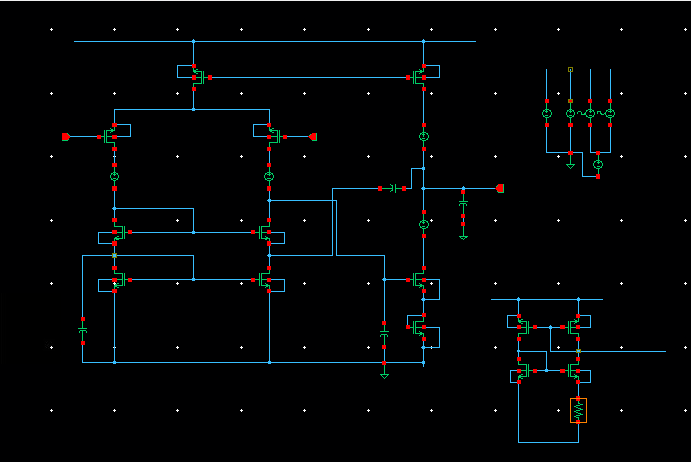
\includegraphics[width=1\textwidth]{Capitoli/whole2.png}
\raggedright



Since we were asked to reduce the power consumption, we needed to use a different compensation technique.

We decided to use the Ahuja compensation technique embeeding the current buffer in the first stage , in order to use the already existing current to bias the current buffer.

\section{Gain, Bandwith and Stability}

\subsection{Gain} % (fold)
\label{sec:gain}

For the gain , the current buffer will act as cascode for the active load of the input pair improving the gain.

For this design we decided to split the gain in the following way:

\begin{equation}
	G_{1^{st}_Stage}=286 \ \ \ \ \ \ \ \ 
	G_{2^{nd}_{Stage}}=35
\end{equation}


For the first step we neglect the contribution of the cascoded load considering only $R_{01}$ as load.

We obtain $L_1=1.5 \mu m$ , but it turns out that with this sizing , the contribution of the cascoded load in parallel to $R_{01}$ lead us out of the specification.

At the end we decided to set $L_{1,2} = 1.6 \mu m$ which gives us a gain of 300.

For the moment we set $L_3=L_4$ to the minimum length.

We set the Overdrive voltages as :

\begin{itemize}
	\item $V_{ov_1}=V_{ov_2}=0.2$ to have the maximum transconductance, in order to maximize the gain and reduce the noise of the mirror.

	\item $V_{ov_3}=V_{ov_4}=0.4$ in order to minimize the input referred noise contribution of the mirror couple.

	\item $V_{ov_5}=0.2$ we made this choice in order to use the same reference used by the second stage , this will let us to have only one reference generation circuit.

	\item $V_{ov_cas1}=V_{ov_cas2}=0.2$ , the lower possible in order to not degrade the common mode input voltage range.

	\item $V_{ov_6}=V_{ov_7}=0.2$ to have our amplifier almost rail-to-rail.

\end{itemize}


\centering
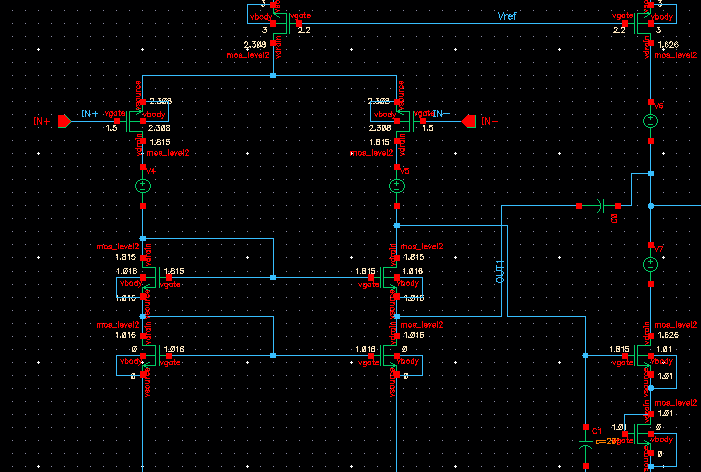
\includegraphics[width=0.6\textwidth]{Capitoli/dc.png}
\raggedright


\subsection{Bandwith} % (fold)
\label{sub:bandwith}

As in the previous design ,starting from the GBWP specification and assuming for the moment $C_c=1pF$ we get $g_{m1}= 250 \mu S$ 

\centering
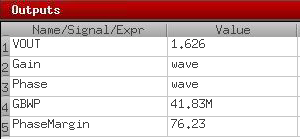
\includegraphics[width=0.7\textwidth]{Capitoli/gnp.png}

\raggedright



% subsection bandwith (end)

\subsection{Phase Margin} % (fold)
\label{sub:phase_margin}

The compensation technique will not change the frequency of the first pole, and from the simulations it's evident the presence of an in-band doublet, taking as to 76.23 of phase margin.


It turns out by the simulation that we cannot have the gate of M6 at 0.8V as it's lower limit it's fixed at 1.2V by the saturation of $M_{CAS2}$.
So we decided to add a transdiode between the source of M6 and ground , in order to have a consistent bias accepting a reduction of the output voltage swing\footnote{Which in this case was not a constraint}.

\centering
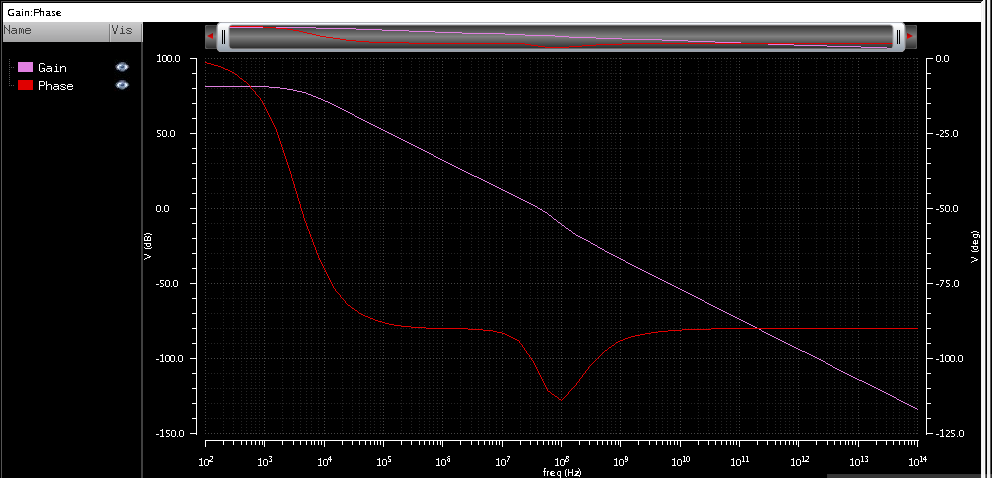
\includegraphics[width=1\textwidth]{Capitoli/gain2.png}
\raggedright


\section{Noise} % (fold)
\label{sec:noise}


\subsection{White Noise} % (fold)
\label{sub:white_noise}

The input reffered noise is going to be same as in stage of part 1 as the transconductance of M1, M2, M3 and M4 were not been modified.

\centering
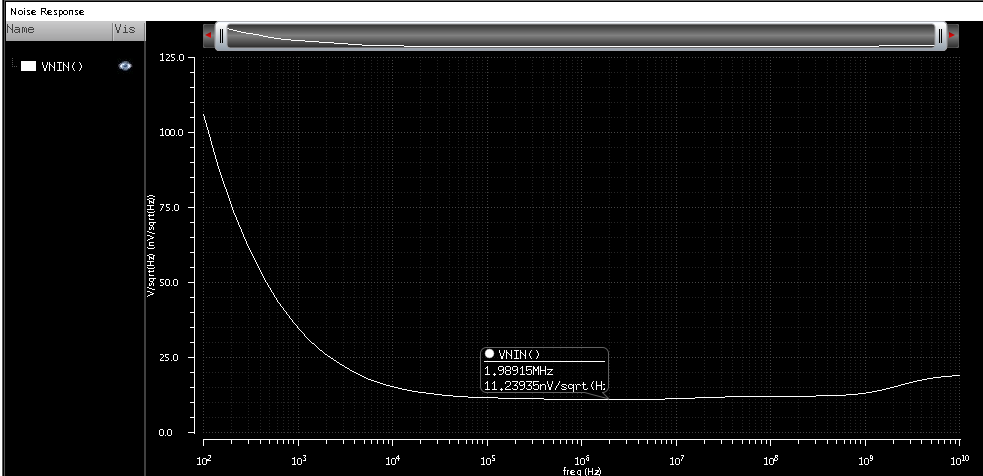
\includegraphics[width=1\textwidth]{Capitoli/wn.png}
\raggedright


\subsection{Noise Corner Frequency} % (fold)
\label{sub:noise_corner_frequency}

The noise corner frequency results to be 8.358KHz and the simulation confirms our result.




\centering
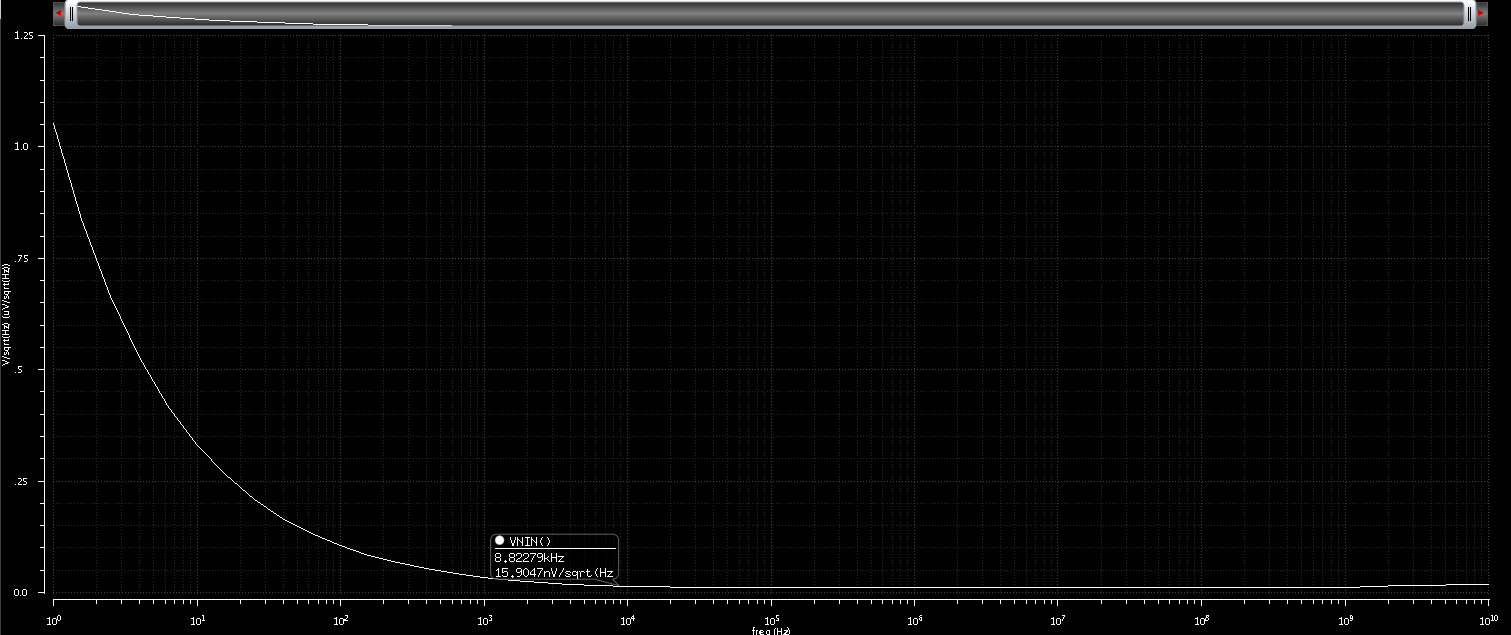
\includegraphics[width=1\textwidth]{Capitoli/ncf.png}
\raggedright


\section{Bangap Reference}


To have our current/voltage reference decoupled, as much as possible, from nominal values of components we used a self biasing circuit derived from tha bandgap topology.


\centering
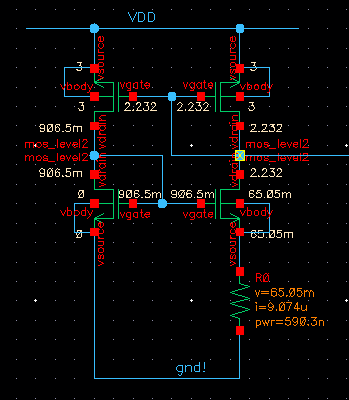
\includegraphics[width=1\textwidth]{Capitoli/bg.png}
\raggedright


In particular for this circuit we set:

\begin{itemize}

	\item $ (\frac{W}{L})_{bandgap-down-DX} = \frac{0.83\mu m}{0.35 \mu m}$
	
	\item $(\frac{W}{L})_{bandgap-down-SX}= \frac{0.7 \mu m}{0.35 \mu m}$
	
	\item $(\frac{W}{L})_{bandgap-up-DX}= \frac{4.067 \mu m}{0.35 \mu m}$
	
	\item $(\frac{W}{L})_{bandgap-up-SX}= \frac{4.067 \mu m}{0.35 \mu m}$

	\item $R_{ref} = 7.168 K \Omega$

\end{itemize}

% subsection noise_corner_frequency (end)
% subsection white_noise (end)
% section noise (end)
% subsection phase_margin (end)_sub
% subsubsection _sub (end)
% section gain (end)

\section{Testbench}

\centering
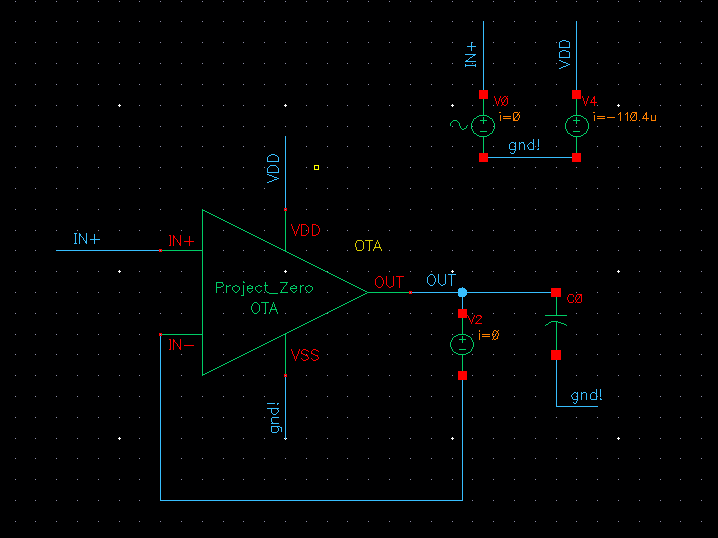
\includegraphics[width=0.8\textwidth]{Capitoli/tb.png}
\raggedright



To verify the performance of our final stage we try to use it in buffer configuration and this are the results:

As we expected using the ahuja compensation topology we can have some decoupling between the bandwith and the load capacitance:


\centering
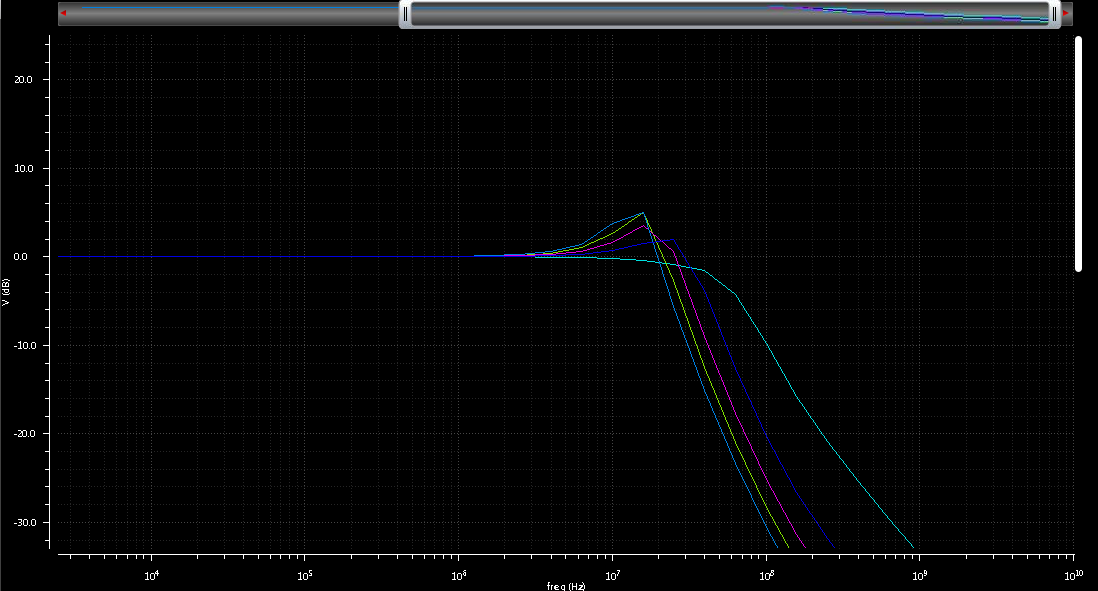
\includegraphics[width=1\textwidth]{Capitoli/cap.png}
\raggedright

\newpage

\section{Results}

\centering
\label{my-label}
\begin{tabular}{|l|l|l|l|}
\hline
\#      & W         & L     & I      \\ \hline
M1 M2   & 40u       & 1.6u  & 19.42u \\ \hline
M3 M4   & 10.9375u  & 3.5u  & 19.42u \\ \hline
M5      & 17.5u     & 0.35u & 38.84u \\ \hline
M6      & 17.5u     & 0.7u  & 38.71u \\ \hline
M7      & 35u       & 0.7u  & 38.71u \\ \hline
M-cas    & 4.375u    & 0.35u & 19.42u \\ \hline
M-diode  & 2u        & 0.35u & 38.71u \\ \hline
M-BG-DW-SX & 0.7u      & 0.35u & 10.62u \\ \hline
M-BG-DW-DX & 0.831u    & 0.35u & 9.074u \\ \hline
M-BG-UP-SX & 4.067u    & 0.35u & 10.62u \\ \hline
M-BG-UP-DX & 4.067u    & 0.35u      & 9.074u \\ \hline
R-ref      & 7.168kohm &       &        \\ \hline
\end{tabular}


\begin{equation}
  E_n^2=( 11.51 \frac {nV} { \sqrt{HZ}})^2
\end{equation}

\begin{equation}
  \phi_m=76.23
\end{equation}

\begin{equation}
  GBWP=41.83MHz
\end{equation}

\begin{equation}
  Gain=80.34dB
\end{equation}
% section results (end)

\begin{equation}
  Current \ \ Consumption = 97.24 \mu A
\end{equation}



% chapter part_2 (end)